%Experimental body
%Created MB 04-12

\section{Experimental}\label{experimental}

\subsection{Apparatus}\label{apparatus}

The goal of the experimental apparatus is to create a robust system in which atoms can interact with electromagnetic fields in a controlled fashion. A glass cell containing rubidium metal, a chosen buffer gas, and an exchange gas is placed into a cylindrical mu-metal shell with openings at the ends, which serves to shield the experiment from the earth's magnetic field. Inside the cylinder, a resistive element is used as a heater; combined with a high-current power supply and a Hewlett Packard platinum film thermometer inserted into the cell area, the temperature of the apparatus is able to be regulated with a fair degree of accuracy. \footnote{As the thermometer is slightly magnetic, it is important to remove it before taking measurements.} A $12$'' diameter, $27.75$'' long aluminum cylinder inside the shield is wound with $1064\pm4$ turns of enameled wire, creating a uniform magnetic field inside the solenoid. The electromagnet is supplied with current from a set of $6$ C cell batteries, for a combined $9$ V, while a potentiometer allows for control of the current in the range of $5$ to $50$ mA and a $1 \Omega$ series resistor allows for accurate monitoring of the solenoid current. \footnote{Note that the current from the batteries drifts downwards over time, and while great care was taken to ensure a constant magnetic field, ultimately the measurement of the current may vary by as much as $0.03$ mA.} Finally, the shield also houses a set of Helmholtz coils which, when driven by a function generator, will provide the radiofrequency fields for the atoms. The glass cell is placed directly in the center of the Helmholtz coil, allowing for a rather uniform distribution of the field through the pumping region.

The optics of the experiment are set up as in Fig.~\ref{fig:optics1} below: 

\begin{figure}[htbp]
\begin{center}
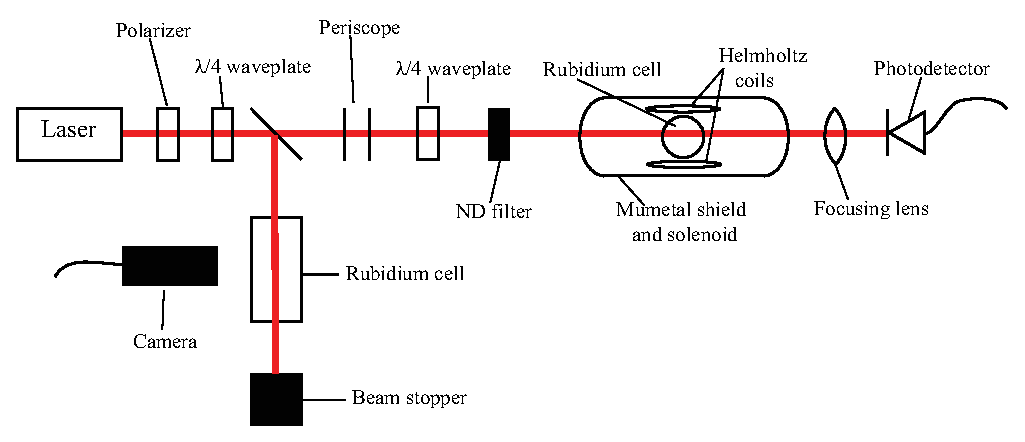
\includegraphics[height=50mm]{./figures/optics1.eps}
\caption{\small{The generic optics arrangement used in this experiment.}}
\label{fig:optics1}
\end{center}
\end{figure}


The laser used in the experiment is a Sharp LT025MD tunable laser diode with grating feedback. Because wavelength increases as a function of temperature and the free-running wavelength of the laser is only $790$ nm and the D1 wavelength is $794$ nm, the laser is operated at approximately $50^{\circ}$ C. A system of thermoelectric coolers and a more fine-tuned temperature control circuit keep the temperature of the laser steady, so as to keep the wavelength of the laser stable.   Adjusting the current supplied to the laser allows for fine control of the wavelength and power of the laser. Note that there is no independent power and wavelength control; furthermore, the laser current drifts down over time. However, as the laser did not drift out of the sensitive region of the rubidium during any of the experiments, this had little effect upon the measurements. Upon leaving the laser housing, the beam is both collimated and linearly polarized.

The next piece of optics the laser encounters is a linear polarizer and a quarter wave plate cemented to the face of a polarizing cube. This combination is used to prevent back reflection into the laser; furthermore, the circularly polarized light is guaranteed to be split $50-50$ by the polarizing beam-splitter cube. 

The diverted beam shines through a small cylinder filled with rubidium vapor before ending at a beam-stopper. A small plastic housing encloses the cylinder and allows an infrared camera to monitor the fluorescence of the rubidium as the laser passes through. By adjusting the laser current and monitoring the fluorescence on a television attached to the camera, it is possible to accurately set the laser to the desired rubidium transition line.

The other part of the beam first encounters a periscope so as to raise the level into the plane of the shielding cylinder. After leaving the beam splitter the laser light is once again linearly polarized, so a quarter wave plate is used to circularly polarize it. The light then encounters an optional neutral density (ND) filter and passes through the cylinder and the rubidium cell; depending upon the magnetic fields present, portions of the laser light will be absorbed. After the beam leaves the cylinder, a lens with a $100$ mm focal length focuses it onto a variable-gain Thorlabs PDA36A photodetector. \footnote{Note that the photodetector is mounted with an $800$ nm interference filter, which enables the experiment to be run with the room lights on and guaranteeing that any light detected is in the neighborhood of the appropriate wavelength.} The signal from the photodetector, which is able to distinguish the various levels of absorption in the rubidium, is then read by a voltmeter or an oscilloscope.

The general system of optical pumping that we observe works as follows: circularly polarized light interacts with the rubidium atoms, and some of them absorb the photons and enter the excited state with $l_{e}=l_{g}+1$ (the sign depending on the polarization direction of the light, but chosen here to be positive for simplicity). The excited atom will spontaneously decay down to any allowed ground state, \emph{i.e.} $l_{g} = l_{e} \pm 1$. However, the atoms in the most extreme $+l$ state will not be able to be transferred to the excited state, as there is no way for them to increase their $l$. As atoms decay from the excited state into allowed ground states equally, the ones that fall into $l=l-1$ will be moved back to the excited state until they decay again. Each time this decay occurs, half the atoms move into the extreme state, and so eventually all the atoms will be in this state. Experimentally, this is observable as an increase in the transmission of the laser through the atoms, as the light is not absorbed when the atoms are in the extreme, ``dark'' state. 

\subsection{Direct Signal Measurements}\label{directsignalmeasurements}

The goal of the first group of experiments was to determine the transient behavior of the atoms as the solenoid field is turned on and off, and to understand the Rabi oscillations present when the radiofrequency magnetic field is applied. The current applied to the solenoid was $19.93$ mA.

The study of the transient behavior was performed by first tuning the laser to the appropriate transition and setting the oscilloscope trigger level appropriately. As the solenoid magnetic field is turned on, the hyperfine states of the atom split and optical pumping becomes possible, and therefore transmission of the laser goes up as more atoms are put into a ``dark'' state that cannot absorb the circularly polarized light. By studying the oscilloscope trace, it is possible to estimate the optical pumping time associated with the atoms and the given light intensity. Furthermore, by studying the decay of the signal after the magnetic field is turned off, it is possible to estimate the relaxation time of the atoms' spin, $T_{1}$. Both of these measurements are approximate at best, because of the finite time in which the magnetic field actually turns on and off. \footnote{More complete measurements are described in Section \ref{measurementoft1}.} However, because of the simple procedure, the data is still worth taking and comparing to more correct measurements.

To study the Rabi oscillations, the function generator was set to create a radiofrequency wave, amplitude modulated from $0$ to $100\%$ at a frequency of $21$ Hz. With this rate of chopped signal, it was possible to trigger the oscilloscope on the frequency generator's sync signal and to time average over repeated cycles so as to minimize noise. All data was taken on a SOMETHING SOMETHING oscilloscope.

\subsection{Measurement of $T_{1}$}\label{measurementoft1}

To measure $T_{1}$ more accurately, it would be ideal to turn off the optical pumping laser instantaneously, let the atoms evolve in the dark for a chosen time period, and then measure the transmission of the laser through the atoms. As the atom spins decay to a thermal distribution, more atoms will be able to absorb the circularly polarized light, and transmission of the laser will decrease. As the laser optically pumps the atoms, the transmission will once again increase, but at the instant that the laser is applied, the transmission level provides accurate information about the distribution of the ``dark'' state of the atoms. Furthermore, the rise of the transmission will provide an accurate measurement of the optical pumping rate of the atoms. The question, then, is how to instantaneously turn off the laser for variable lengths of time.

The solution is a Stanford Research Systems SR540 optical chopper. By placing the chopper in the middle of the beam as in Figure SOMETHING it is possible to regularly turn on/off the beam at a chosen frequency. However, as the beam is rather wide when it leaves the laser, it is necessary to use a series of $16$ mm focal length lenses to focus the beam at the chopper and then expand it back to size: otherwise, the chopping time would be finite, as the beam was slowly covered by the surface of the chopper. The modified optics diagram is displayed in Fig. \ref{fig:optics2}. \footnote{The beam is re-expanded so as to be able to interact with a larger cross-section of atoms in the glass cell.} The signal from the photodetector is monitored on an oscilloscope and analyzed as discussed above. At higher chopping frequencies, it is possible to trigger and time average on the oscilloscope, reducing signal to noise. \footnote{The averaging is not possible to perform at lower frequencies, as the chopper is very slightly damaged and does not spin perfectly evenly. This effect is only visible at lower frequencies, as at higher frequencies the chopper spins so quickly that the effect is not noticeable.}


\begin{figure}[htbp]
\begin{center}
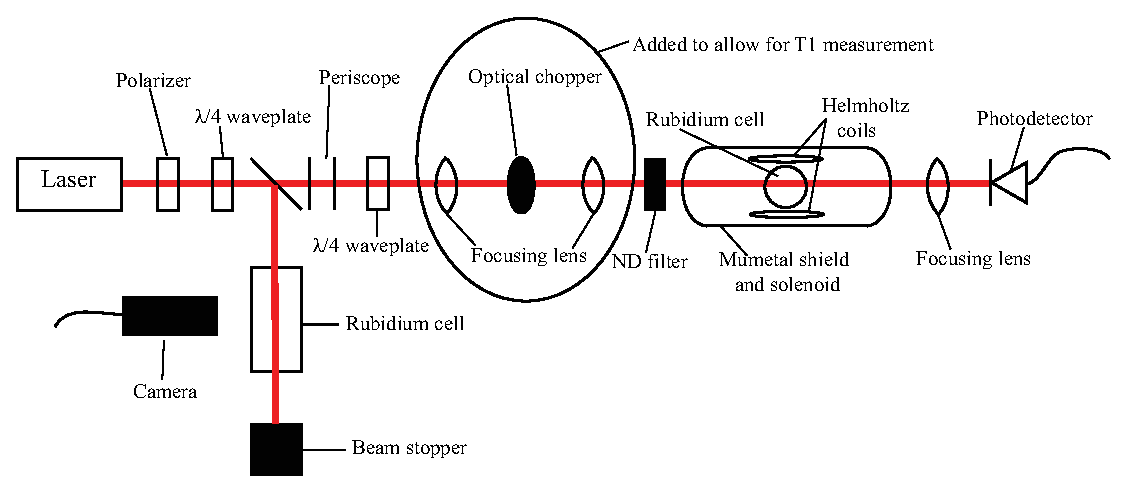
\includegraphics[height=50mm]{./figures/optics2.eps}
\caption{\small{The modified optics arrangement used to measure $T_{1}$.}}
\label{fig:optics2}
\end{center}
\end{figure}


Note that at higher frequencies, the signal will be chopped before the atoms have reached the completely pumped state, and so the transmission level they start from will be lower than the equilibrium at lower frequencies. To normalize, for each frequency the measurement performed is of the ratio of the transmission after the dark period to before. The measurements were all performed on the $3\rightarrow3$ $^{85}$Rb transition, as the $^{87}$Rb value is much more difficult to measure because of the lower concentration of this isotope in the cells we used.

\subsection{Measurement of $T_{2}$} \label{measurementoft2}

To gain a better understanding of the properties of the atom, it is also desirable to measure the $T_{2}$ of the atom: \emph{i.e.} the rate at which the atomic spins lose coherence. As derived in section SOMETHING, the linewidth of the Lorentzian is inversely proportional to the $T_{2}$ time of the atoms. The principal experimental difficulty is the power-broadening of the linewidth at high radiofrequency signals and high laser intensities. In the limits where the other broadening factor does not contribute, we have as derived in sections BLAH and BLAH, we have:

\begin{eqnarray}
\gamma_{m} &=& \gamma \sqrt{1+ \kappa_{rf} B^{2}} \label{eq:rfbroad}\\
\gamma_{m} &=&\gamma \sqrt{1+ \kappa_{las} \mathcal{E}_{0}^{2}} \label{eq:lightbroad}
\end{eqnarray}

where $\gamma_{m}$ is the measured linewidth, $\gamma$ is the real linewidth, $B$ is the amplitude of the radiofrequency fields, $\mathcal{E}_{0}^{2}$ is the intensity of the laser, and the $\kappa$ factors are constants. Combining the equations is a complicated matter which requires a full derivation of the three-state system, so we consider the effects separately by measuring them in the limits where the other factor has reached the asymptote. The goal, then, is to measure the linewidth as independent functions of radiofrequency amplitude and light intensity and extrapolate both back to the asymptotic region where the broadening factor does not contribute.

To measure the linewidth, we record the amplitude of the the Rabi oscillations at different rf frequencies, with the rf signal chopped as described in Section \ref{directsignalmeasurements}. To increase signal to noise when measuring this amplitude, a lock-in amplifier is synced to the function generator, and the resulting signal is read by a voltmeter. A LabView program interfacing with the function generator and the voltmeter steps through different frequency settings and records the amplitude after a given averaging time.

To find the function dependent on rf amplitude, we insert a strong ND $2.0$ filter so as to remove SOME $\%$ of the light. \footnote{We guessed that this would be low enough intensity that the signal was not broadened; later results proved this correct, but if they hadn't, we would have repeated this experiment with a higher strength ND filter.} The LabView program can also control the peak-to-peak voltage of the function generator, allowing the linewidth to be recorded at many different voltage levels. This data is fit to Eqn. \ref{eq:rfbroad}, allowing for $\gamma$ to be calculated. Note that between measurements it is important to realign the laser to the appropriate transition, as the laser tends to drift slightly off over long periods of time. This has little effect on actual data runs, but would compound over multiple measurements.

The procedure for measuring the dependence on the light intensity is very similar. From the fit above, a value of the radiofrequency amplitude low enough to be in the asymptotic region is selected. Then, the ND filter is adjusted in increments of $0.1$ and the linewidth recorded using the LabView program. The resulting linewidths are fit to Eqn. \ref{eq:lightbroad} and extrapolated to 0 intensity.  Note that this plot confirms that an ND value of $2.0$ is in the asymptotic region, so our selection in the original experiment was acceptable.

This procedure was performed on the $3\rightarrow3$ transition in $^{85}$Rb. The rf measurement was also performed with an ND of $2.0$ (again, sufficiently high to be safe) on the $2\rightarrow2$ transition in $^{87}$Rb. Thus, we were able to measure the $T_{2}$ time for both isotopes of rubidium. Whereas the difference between $T_{1}$'s is not particularly interesting and was therefore omitted, the difference here is related to the different spin-exchange rates of the two isotopes.

\subsection{Measurement of $^{85}$Rb and $^{87}$Rb Spin-Exchange Rate}

One of the factors contributing to the $T_{2}$ relaxation time are spin-exchange collisions between the different gasses in the cell. It is possible to measure this rate by shining the laser on say, a $^{85}$Rb transition, and driving the radiofrequency at the $^{87}$Rb rate. The $^{87}$Rb will be undergoing Rabi oscillations and will transfer their spins to the $^{85}$Rb at each point of the oscillation, as discussed in section BLAH. Because of these spin exchanges, the $^{85}$Rb will be effectively undergoing Rabi oscillations, and we should be able to measure the normal Lorentzian distribution at around the $^{87}$Rb rf frequencies, even though the $^{87}$Rb is not being optically pumped. The linewidth here will correspond, just as in previous experiments, with a power-broadened natural linewidth:

\begin{equation}
\gamma_{m} = \gamma_{se} \sqrt{1+\kappa_{rf} B^{2}} \label{eq:sebroad}
\end{equation}

The resonance of the $^{85}$Rb at the frequencies which correspond to $^{87}$Rb can be due to only the spin-exchange mechanism, so it is natural to call the unbroadened linewidth $\gamma_{se}$, the spin-exchange rate. Furthermore, we expect power-broadening of the same rf form as we've seen before: a larger rf amplitude will increase the rate of coupling, and there should still be coupling with no radiofrequency field. Note that because of the different concentrations of rubidium isotopes, the spin-exchange rates will not be symmetric; \emph{i.e.}, because there is little  $^{87}$Rb, driving this frequency will have a very small effect on the $^{85}$Rb, whereas driving on the  $^{85}$Rb rf frequencies will have a much larger effect on the  $^{87}$Rb.

Experimentally, the primary obstacle in this measurement is this very low strength of the coupling and therefore the very low amplitude of the measured oscillations. To compensate, the sensitivity of the lock-in amplifier is set to $20 \mu$V here, up from $5$ mV in the previous experiments. A 2.0 ND filter ensures that there is no power-broadening due to light, and measurements are performed using the LabView program at different radiofrequency amplitudes. The data is fit to Eqn. \ref{eq:sebroad} and extrapolated to 0 amplitude, allowing for a calculation of $\gamma_{se}$. The measurement is performed on the $3\rightarrow3$  $^{85}$Rb transition and the $2\rightarrow2$ $^{85}$Rb transition. 

\subsection{Measurement of Rubidium $g$-factor}

As discussed in Section BLAH, the peak of the Rabi oscillation amplitudes occurs at the frequency corresponding to the Zeeman splitting of the magnetic sublevels. By measuring this frequency and calculating the magnetic field of the solenoid, it is possible to calculate the $g$-factor of the atom, according to equation SO AND SO.

The calculation of the magnetic field is straightforward when the solenoid properties and current are known. To measure the peak frequency, the LabView program is used to produce the spectrum at several different radiofrequency amplitudes. The maximum frequency should not move because of power-broadening, so the center of these curves are averaged and this value is chosen as the splitting frequency. This measurement is performed on all of the available rubidium splittings.











